\documentclass[10pt, conference, compsocconf]{IEEEtran}
\usepackage{csquotes}
\usepackage{epigraph}
\usepackage{graphicx}
\graphicspath{ {graphics/} }
\renewcommand\IEEEkeywordsname{Keywords}
\renewcommand{\figurename}{Figure}

\begin{document}

\title{Adaptive Indexing: Cracking Facts and Merging Knowledge}
\author{Pavlo Shevchenko \\ Otto-von-Guericke-University, Magdeburg \\ pavlo.shevchenko@st.ovgu.de}

\maketitle

\epigraph{Therefore, even as an index to a book \\
So to his mind was young Leander's look}{\textit{Christopher Marlowe\\Hero and Leander, 1593}}

\begin{abstract}
What did I do in a nutshell?\\
\end{abstract}

\begin{IEEEkeywords}
Database indexing, adaptive indexing, database cracking, adaptive merging, hybrid approaches.
\end{IEEEkeywords}

\section{Introduction}
The concept of indexes was widely used in bibliothecography throughout the history of mankind. %First reference to indexes in the English language is to be found in Christopher Marlowe's \textit{Hero and Leander}, 1593 [1]:
%\begin{displayquote}
%Therefore, even as an index to a book \\
%So to his mind was young Leander's look
%\end{displayquote} 
Indexes designed to help the reader find information quickly and easy found their way into the databases. Introduction of such intuitive concept helped to improve the speed of data retrieval. In the early stages of database technology data and indices were stored on disk in a form of B-Trees.

However, over the years, as in-memory databases (IMDB) found their way to the market, need for more lightweighted index structures has become evident. At first, precalculated index in a form of a sorted column with pointers to the original records in the table has become a concept that helped to decrease the query response time. However, continuously growing amount of data, more sophisticated queries and unpredictable behavior of a user have turned advantages of indexes into disadvantages. Storing large columns in a main memory has become a problem, need to store indexes to numerous columns has even increased that problem. As it was hard to predict which column is especially interesting for the user, new indexes have to be calculated online as queries referring to new columns arrive.

All these issues motivated development of advanced indexing techniques as \textit{partial} \cite{partial1} and \textit{soft} \cite{soft_indexes} indexes. We discuss both these concepts in details in Background section. Creators of the latter, L\"uhring et. al., have predicted the future of database indexes. They realised that index cannot remain static after being created, it requires to be continuously tuned as some parameters of database system are changing. Such parameters include workload, size and distribution of data, schema and infrastructure changes  \cite{soft_indexes}. This leads to a conclusion that the best index is a result of query processing with all these parameters kept in mind.

This concept known as adaptive indexing will be presented in this short paper. We revisit some fundamental approaches (e.g. database cracking \cite{cracking} and adaptive merging \cite{merging}) in Sections 3 and 4 respectively. Further approaches that try to combine the advantages of both methods will be introduced in Section 5. We evaluate presented approaches in Section 6. We conclude this paper by presenting related work in Section 7 and proposing directions for further reasearch in Section 8.

Our goal is to provide a complete overview of adaptive indexing techniques to help everyone interested in them understand core concepts of the approaches. Furthermore, we aim to draw attention to these techniques and motivate further studies in the area of adaptive indexing.

\section{Background}
As mentioned before, two indexing methods: partial indexes \cite{partial1} and soft indexes \cite{soft_indexes} were developed to tackle some problems caused by traditional indexes. In this section, both of these approaches and their influence on adaptive indexing will be presented.
\subsection{Partial Indexes}
As its name suggests, partial index, also known as filtered index, is an index which contains only part of the indexed column that satisfies some condition. Such condition is usually expressed in a form of an interval known as \textit{inclusion interval}. Depending on selectivity of a condition, the amount of rows in the indexed column can be decreased. This allows to reduce the amount of memory needed to store the index. Creation of such index may be specified as follows:
\begin{displayquote}
\texttt{CREATE \hspace{0.2 cm} INDEX \hspace{0.2 cm} ON \hspace{0.2 cm} relation(column) name \\ WHERE \hspace{0.2 cm} condition}
\end{displayquote}

In Figure 1, we present an example of a partial index with a condition $'D' \leq A \leq 'O'$. Next to it, we give an example of a full index to a given table.

Clearly, selecting the right condition is a key element for creation of partial index. Condition can be found in several ways:\\
\begin{itemize}

\item{User Input:}\\ Obviously, user can specify the insertion interval while possessing some additional knowledge about the data. However, one of the major principles of modern DBMS is removing any low-level data management aspects from the user of the system. As a result, some database tuning is needed.\\

\item{Index Creation as Side-Effect of Query Processing \cite{partial1}:}\\ Even though user has been removed from tuning process, consumer can still indirectly participate in finding a suitable condition. The fact that user queries some relation (column) while applying some selection condition, leads to an assumption that this part of data is of some interest for the user and may be queried again in the future. So, taking query condition from the user as a qualification for partial index is not a bad idea after all. Continuous refinement of a condition and index ad hoc may provide an optimal partial index for given relation. This concept was later used in database cracking.\\

\item{Statistical Approach \cite{partial2}:} \\Since index creation in a way described above may increase query processing time, statistical information, like the percentage of queries that access each column or distribution of values iin each column, may be used to perform index creation after data loading and before queries are processed.
\end{itemize}

\begin{figure}[h]
\centering
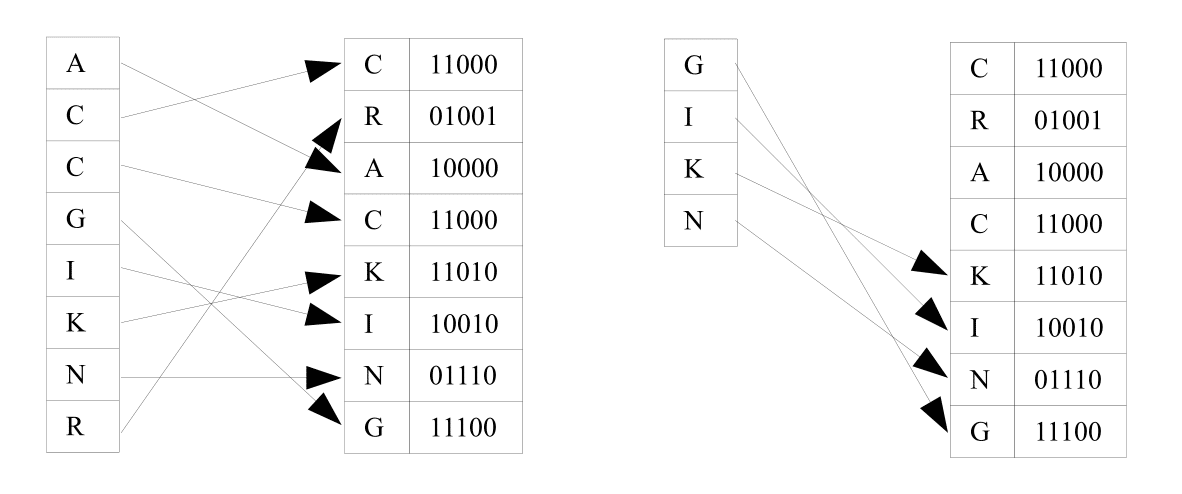
\includegraphics[width=\columnwidth]{partial.png}
\caption{Full Index (left) and Partial Index (right)}
\end{figure}

\subsection{Soft Indexes}
Soft indexes proposed in \cite{soft_indexes} is one of the first attempts to pass responsibility for index creation from DBA to DBMS. Index management is carried out in three major steps:
\begin{itemize}
\item{Observation}
\item{Prediction}
\item{Reaction}
\end{itemize}

At first, statistical information about current state of the system (workload, data, schema, infrastructure) is collected (Observation). Afterwards, in order to derive an optimal index configuration, a list of index candidates sorted by some criteria is analyzed and top \textit{k} candidates are chosen for materilization in the Reaction phase. During the latter, depending on results of Prediction phase, some indexes will be created or deleted \cite{soft_indexes}.\\

\textbf{Meaning}. Combination of advantages of soft and partial indexes resulted in further approaches known as adaptive indexing. On-the-fly index creation based on query workload and storing only subset of rows in an index motivated the first method for adaptive indexing, called \textit{database cracking} \cite{cracking}, which we present in the next section.

\section{Database Cracking}
After presenting the necessary background about partial and soft indexes, we revisit one of the main approaches of adaptive indexing, database cracking. In Subsection A we discuss main idea behind database cracking, in Subsection B we revisit standard cracking algorithm. In Figure 2, we show work of previously described algorithm on an example. To conclude this section, we analyze database cracking and compare it to full index and full scan.

\subsection{Motivation and Basic Idea}
\textbf{Motivation}. Database cracking is pursuing the goal to provide fast access to the data and the self-organized behavior of database system. It is based on idea that index maintenance is a byproduct of query processing, not updates \cite{cracking}. In contrast to soft indexes, discussed earlier, database cracking achieves its goal not by tuning system's configuration and choosing the best fitting indexes based on numerous parameters, but by using continuous physical reorganization (cracking the database into manageable pieces).

\subsection{Standard Cracking}
\textbf{Main Idea}: \textit{incrementally perform quick sort on a copy of a column using crack-in-three when range query fully falls in the same partition and crack-in-two otherwise.}\\

\textbf{Crack-In-Two}: \textit{partition the index column into two pieces using range as a split line.}\\

\textbf{Crack-In-Three}: \textit{partition the index column into three pieces using ends of a range as two split lines.}\\

\textbf{Steps of Standard Cracking} (given a column oriented database with column \textit{A}; range query \textit{q} in a form of either \textit{$c \leq R.A$} or \textit{$c_1 \leq R.A \leq c_2$}): \\
\begin{enumerate}
\item{Initial Index Creation:}\\
The first time query on attribute \textit{A} arrives, copy of the column is created and cracked using \emph{Crack-In-Two} or \emph{Crack-In-Three} (notation:  $A_{crk}$). This allows to leave original column intact and fast reconstruction of records. \\
\item{Refinement:}\\
As further queries on attribute $A$ arrive, partition $A_{crk}$ with regard of earlier cracking. E.g. $q_1 = 5 \leq R.A \leq 10$. After cracking, $A_{crk}$ will contain three partitions as described earlier. When next query arrives $q_2 = 7 \leq R.A$, then cracking should be performed only on part of $A_{crk}$ between positions $p_1$ and $p_2$, as it is known that all elements before position $p_1$ satisfy the query and all elements after $p_2$ don't.\\
\item{Cracking Index:}\\
In order to quickly find the partition to be refined, each cracker column is provided with \textit{cracker index} which stores how values are currently distributed in the cracker column. Each node of a tree stores key value, start position of a partition with this key, and whether key itself is included in the range or not.\\
\item{Query for new column $B$ arrives}\\
Perform steps 1 through 3 for new column $B$ and store previous results.
\end{enumerate}

\begin{figure}[h]
\centering
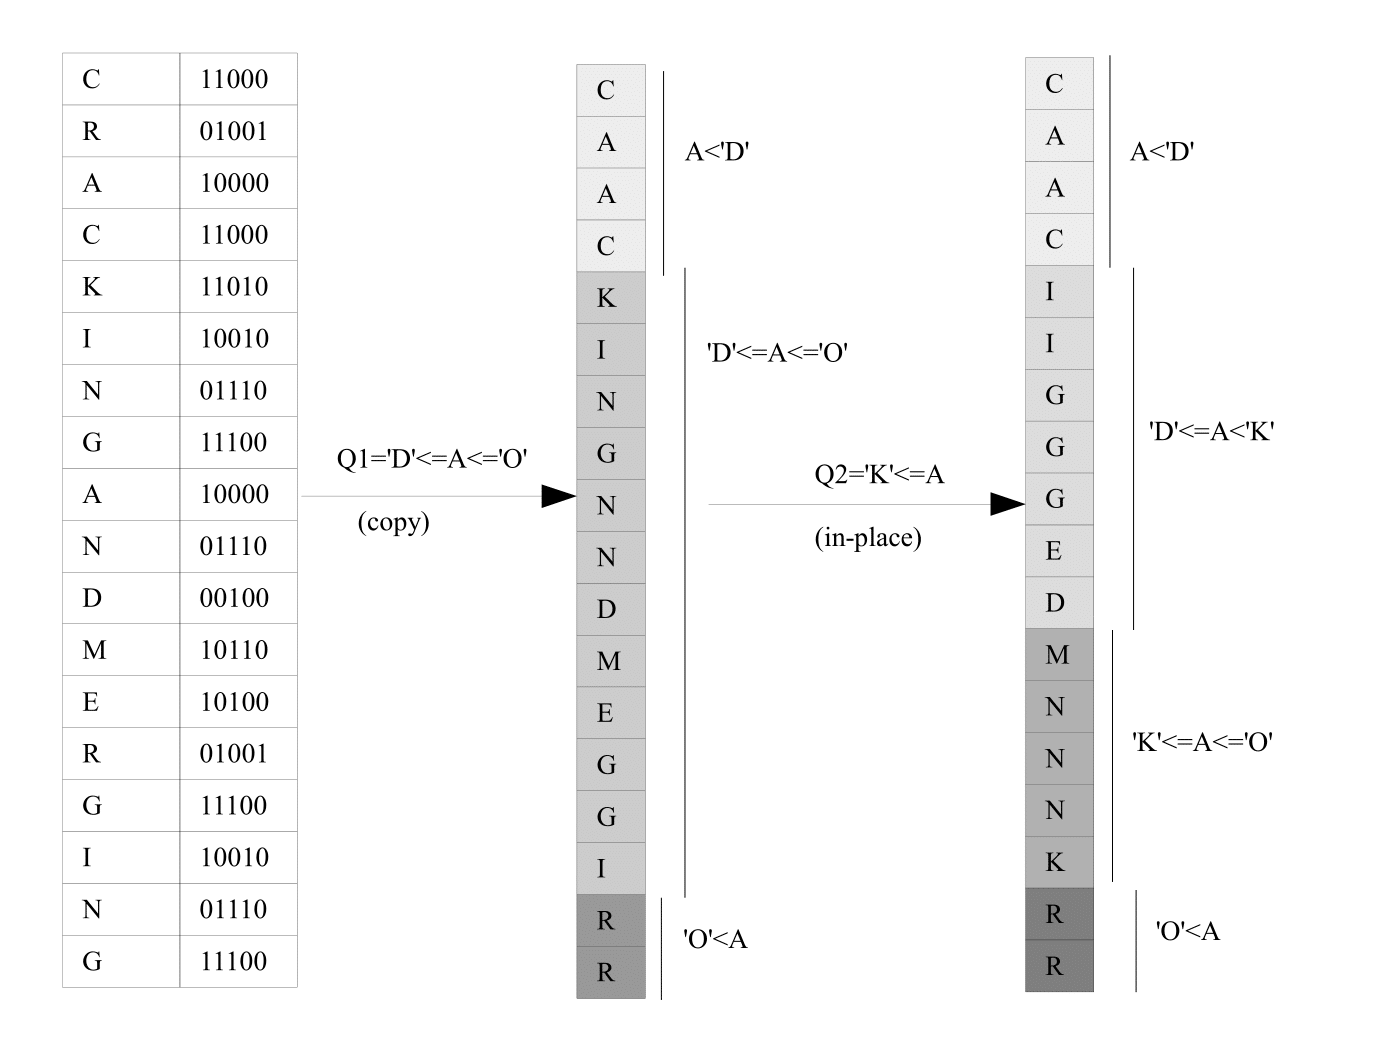
\includegraphics[width=\columnwidth]{cracking.png}
\caption{Cracking a column (adapted from \cite{cracking})}
\end{figure}

\subsection{Analysis and Criticism}
\textbf{Analysis}. In order to analyze database cracking, we compare this approach to full index and full scan.\\
\begin{itemize}
\item{Costs of Initial Run:} \\High creation costs are the main concern of full index. While using full index, query processing can start only after initial index creation. Database cracking offer significant imporvements to avoid full sort of index column. Initial run happens as the first query arrives. In general, first crack takes longer than full scan, as cracking invests some time in indexing. However, cracking still needs less time for initial run than full index to sort the data \cite{survey_cracking}.\\
\item{Costs of Query Processing:} \\After being created, full index processes new queries fast, utilizing advantages of index structures. Full scan takes on average same time to process each next query as it scans the whole table to find relevant tuples. Apart from first query, database cracking performs better than full scan and incrementally reaches the performance of full index \cite{survey_cracking}.\\
\item{Convergence Towards Full Index:} \\As mentioned in previous point, database cracking constantly narrows its performance towards full index. It is achieved by incrementally sorting the cracked column when new queries arrive. Consequently, cracked column converges towards full index after number of queries. Clearly, the quality of cracking step highly depends on the split line defined by query's range. Thus, it is hard to predict how soon query response time of cracking will be reasonably close to one of full index. On average, after 1,000 queries, query response time of standard cracking is still about 40\% higher than of full index \cite{eval2}.\\
\end{itemize}

\textbf{Criticism}. Several weaknesses of database cracking were outlined in the past. Apart from slow convergence towards full index, they include unpredictable query response time, worse performance with growing number of projected attributes, and not suitable implementation for block-access storage. In \cite{survey_cracking}, Schuhknecht introduced several approaches such as Vectorized, Hybrid, Sideways and Stochastic cracking, that try to solve these problems. However, one of the key problems of database cracking: slow convergence, remains unsolved. This concern motivated the development of further adaptive indexing method: \textit{adaptive merging}, which we present in next section.

\section{Adaptive Merging}
In Section 3, we presented a pioneer approach for adaptive indexing, known as database cracking. We outlined some issues related to this method. In following subsections, we present another adaptive technique for index creation, known as adaptive merging, that tackles unsolved issues of database cracking \cite{merging}. In Subsection A, we present motivation and main idea behind adaptive merging. In Subection B, we describe the approach, followed by an example in Figure 3 and in Subsection C, we conclude the section with some analysis of this method.

\subsection{Motivation and Basic Idea}
\textbf{Motivation}. Creators of adaptive merging, Graefe and Harumi, outlined four main weaknesses of database cracking that motivated their research \cite{merging}:
\begin{enumerate}
\item{Slow convergence towards full index.}
\item{Efficiency of cracking depends on query pattern.}
\item{Query response time never reaches that of full index, when cracked column has minimal number of unsorted partitions.}
\item{Database cracking is is well-suited for in-memory databases but not for block-access storage.}
\end{enumerate}

\textbf{Main Idea}. Graefe and Harumi proposed adaptive merging, new technique that combines the efficiency of traditional B-tree creation with adaptive nature of database cracking. As its name suggests, adaptive merging is based on merging (as used in merge sort) rather than on partitioning (as used in quicksort and database cracking) \cite{merging}. This new technique promises better query response time and quicker adaption to new data and new query patterns that database cracking.

\subsection{Adaptive Merging}
\textbf{Main Idea}: \textit{exploit partitioned B-trees \cite{partitionedtrees} by merging key ranges relevant to actual queries, aiming to reach desired state and have only a single partition.}\\

\textbf{Steps of Adaptive Merging} 
\begin{enumerate}
\item{Index Selection:}\\
If a column is referred by query for the first time, a new index is created by copying values of a column. \\
\item{Initial Index Creation:}\\
These values are loaded into number of sorted partitions of predefined size. \\
\item{Index Refinement:}\\
When a column is used for the second time, the query scans one or multiple partitions for desired key range. It is done by efficiently finding the low end of the range and then scanning to the high end. Several sorted streams of values, resulting in this step, will be merged into a single sorted stream that will be written into a new partition. Moreover, this stream is returned as a result of given query.\\
\item{Overlapping Key Ranges:}\\
Same as in database cracking, ranges of further queries may be fully included in already existing partitions, lay outside of them, or only part of new range is included in existing partitions. Following strategy is applied in these cases:
\begin{itemize}
\item{New query range is a subset of previous query: }
Peform efficient search in a partitioned B-tree.\\
\item{New and old query ranges do not overlap: }
Perform Step 3, create new partition and return it as a result.\\
\item{New and old query ranges partially overlap: }
Split new range into overlapping and non-overlapping sub-ranges. For overlapping subranges perform search in a partitioned B-tree. For non-overlapping subrange perform Step 3 and create new partition for further queries.\\
\end{itemize}
\item{Storage of Reorganization Information:}\\
Like in database cracking, some data structure is requiered to retain information about performed reorganization. In contrast to Cracking Index used in database cracking, the data structure in adaptive merging contains a range of identifiers for the partitions in which given range of keys can be found. As numerous partitions can contain given key range, list of partitions with this key range has to be stored.
\end{enumerate}

\begin{figure}[h]
\centering
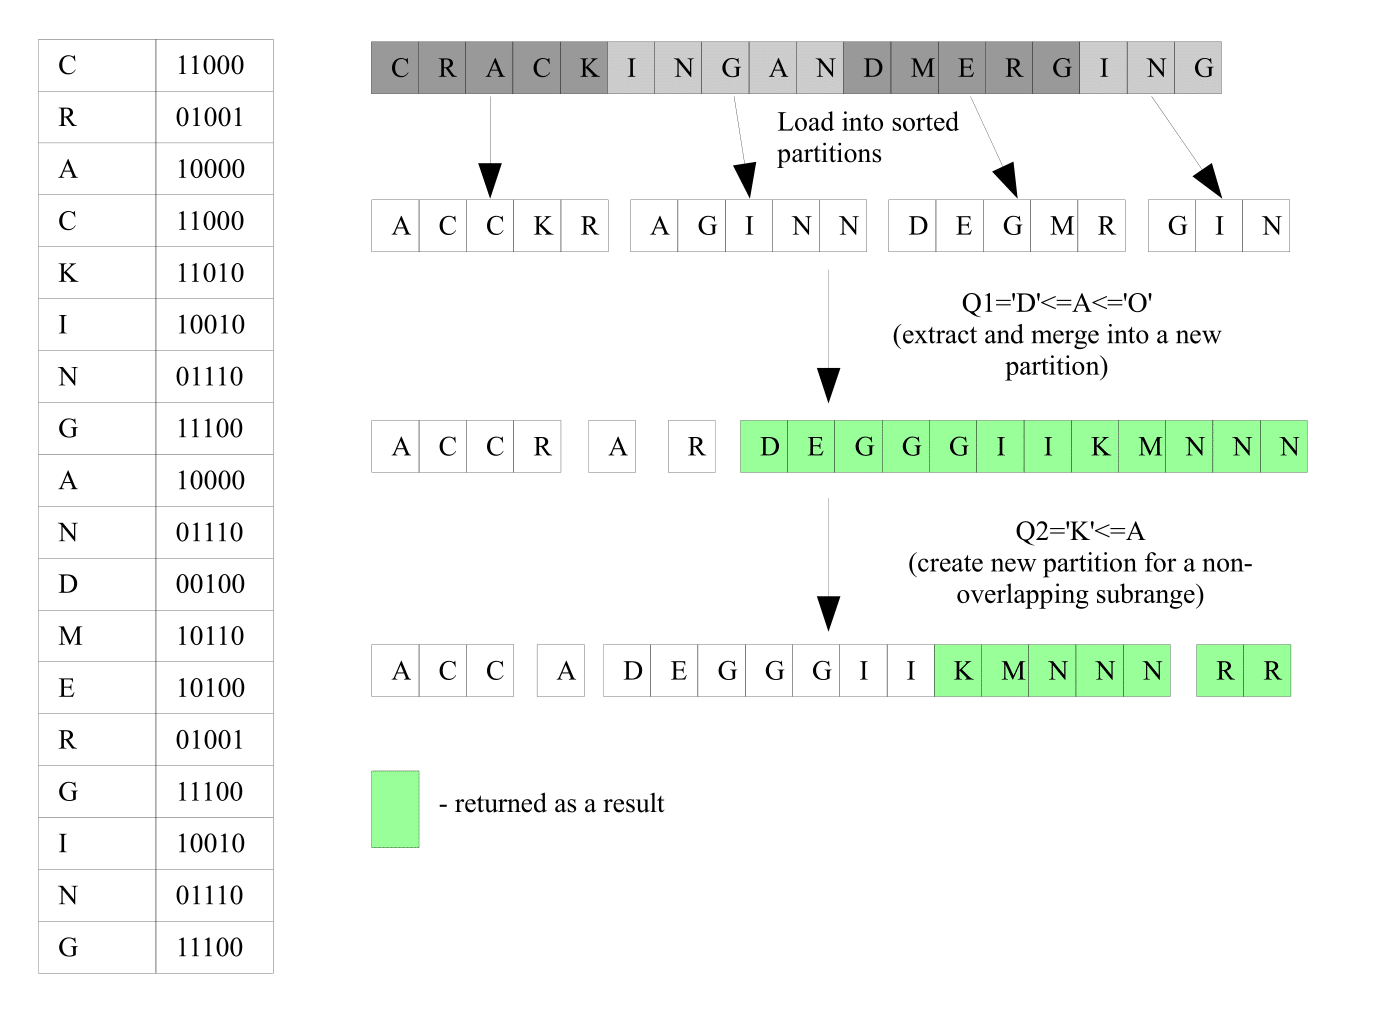
\includegraphics[width=\columnwidth]{merging.png}
\caption{Example for adaptive merging (adapted from \cite{merging})}
\end{figure}

\subsection{Analysis and Criticism}
\textbf{Analysis}. In order to analyze adaptive merging, we compare this approach to database cracking.\\
\begin{itemize}
\item{Cost of Query Processing:} \\Similarly to database cracking, the overhead of first query is large, as the whole domain has to be scanned and partitioned. However, overhead of query processing by adaptive merging decreases faster than that of database cracking. This can be explained by following:\\
\begin{enumerate}
\item{Fast convergence}: In order to divide 10,000,000 records into partitions with appr. 1,000 entries requires at least 9,999 partitioning keys. As each query provides at most two new split lines, to reach this aim, database cracking requiers around 5,000 queries. On the other hand, adaptive merging create a fully optimized B-tree after 40 queries, reaching the behavior of full index \cite{merging}.
\item{Sorted partitions}: Sorted partitions in adaptive merging enable lower query response time even if B-tree is not fully optimized. In database cracking, although new range query may completely lie in already existing partition, cracking must be performed. As partition is unsorted, distribution of relevant elements for new query in existing partition is not known. On the other hand, sorted partitions in adaptive merging enable fast search for the position of a lower key in a partition and scan of entries till higher value.\\
\end{enumerate}
\item{Block-Access Storage:} \\ In contrast to database cracking, designed for in-memory databases, adaptive merging enables adaptive index creation in large data warehouses on external storages. Similarly to traditional B-trees and external merge sort, adaptive merging can be applied to partitioned B-trees and used in block-access storage \cite{merging}. \\
\end{itemize}

\textbf{Issues}. Although adaptive merging matches and may even exceed query response time of full index after a small number of queries, its performance over first queries is concerning. While database cracking mathces the scan performance with the second query and exceeds it after the third, adaptive merging needs around 7 queries to exceed the scan time. The first query may be nearly 5 times slower than a scan \cite{hybrid}.

\section{Hybrid Approaches}

\section{Evaluation}
Point out complementary nature of cracking and merging. Compare to other hybrid approaches. Speculate on future and usage of the methods

\section{Related Work}
Some research on related work has to be done.

\section{Conclusions}
What did I find out?

\section*{Acknowledgement}
I thank M.Sc. Gabriel Campero Durand of Otto-von-Guericke-University, Magdeburg for providing insight and expertise to start this research and for his enormous support throughout the whole process of research, writing and evaluation of this scientific work. I would also like to show my gratitude to the DBSE Research Group of Otto-von-Guericke-University, Magdeburg for making this work possible and organising "Seminar on Modern Software Engineering and Database Concepts", during which this research took place.

\begin{thebibliography}{8}

%\bibitem{first_reference}
%Knight, G. Norman. Indexing, the art of a guide to the indexing of books and periodicals. No. 029.5 K55. 1979.
\bibitem{partial1}
Stonebraker, Michael. "The case for partial indexes." Sigmod Record 18.4, 1989.
\bibitem{partial2}
Seshadri, Praveen, and Arun Swami. "Generalized partial indexes." Data Engineering, 1995. Proceedings of the Eleventh International Conference on. IEEE, 1995.
\bibitem{soft_indexes}
L\"uhring, Martin, et al. "Autonomous management of soft indexes." Data Engineering Workshop, 2007 IEEE 23rd International Conference on. IEEE, 2007.
\bibitem{cracking}
Idreos, Stratos, Martin L. Kersten, and Stefan Manegold. "Database Cracking." CIDR. Vol. 7. 2007.
\bibitem{survey_cracking}
Schuhknecht, Felix Martin. "Closing the circle of algorithmic and system-centric database optimization: a comprehensive survey on adaptive indexing, data partitioning, and the rewiring of virtual memory.", 2016.
\bibitem{merging}
Graefe, Goetz, and Harumi Kuno. "Self-selecting, self-tuning, incrementally optimized indexes." Proceedings of the 13th International Conference on Extending Database Technology. ACM, 2010.
\bibitem{partitionedtrees}
Graefe, Goetz. "Sorting and indexing with partitioned B-trees". CIDR, 2003.
\bibitem{hybrid}
Idreos, Stratos, et al. "Merging what's cracked, cracking what's merged: adaptive indexing in main-memory column-stores." Proceedings of the VLDB Endowment 4.9, 2011.
\bibitem{eval1}
Pirk, Holger, et al. "Database cracking: fancy scan, not poor man's sort!." Proceedings of the Tenth International Workshop on Data Management on New Hardware. ACM, 2014.
\bibitem{eval2}
Schuhknecht, Felix Martin, Alekh Jindal, and Jens Dittrich. "The uncracked pieces in database cracking." Proceedings of the VLDB Endowment 7.2 (2013): 97-108.

\end{thebibliography}

\end{document}
